\documentclass[tikz,border=4pt]{standalone}
\usepackage{amsmath,amssymb}
\usetikzlibrary{arrows.meta}

\begin{document}
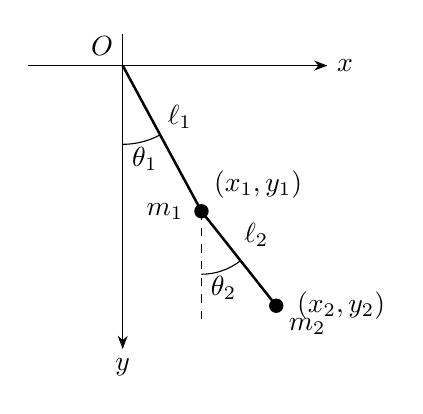
\begin{tikzpicture}[
  >=Stealth,
  font=\normalsize,
  axis/.style={line width=0.4pt},
  curve/.style={line width=0.9pt}
]
  % Axes (y downwards)
  \draw[axis,->] (-1.2,0) -- (2.6,0) node[right] {$x$};
  \draw[axis,->] (0,0.4) -- (0,-3.6) node[below] {$y$};
  \node[above left] at (0,0) {$O$};

  % Mass 1 and Mass 2
  \coordinate (M1) at (1.0,-1.85);
  \coordinate (M2) at (1.95,-3.05);

  \draw[curve] (0,0) -- (M1) -- (M2);
  \fill (M1) circle (2.6pt);
  \fill (M2) circle (2.6pt);

  \node[left=3pt] at (M1) {$m_1$};
  \node[above right=1pt] at (M1) {$(x_1, y_1)$};
  \node[below right=1pt] at (M2) {$m_2$};
  \node[right=4pt] at (M2) {$(x_2, y_2)$};

  % Lengths l_1, l_2
  \node[above right] at (0.45,-0.92) {$\ell_1$};
  \node[above right] at (1.42,-2.42) {$\ell_2$};

  % Angle theta_1
  \draw[axis] (0,-1.0) arc (-90:-61.6:1.0);
  \node at (0.28,-1.18) {$\theta_1$};

  % Vertical dashed line at M1 and angle theta_2
  \draw[axis,dashed] (M1) -- (1.0,-3.25);
  \draw[axis] (1.0,-2.65) arc (-90:-51.6:0.8);
  \node at (1.28,-2.82) {$\theta_2$};
\end{tikzpicture}
\end{document}
